% ==========================================================
%  Pico Handheld Game Console -- Project Report
%  Compile:  pdflatex report.tex   (run twice for the contents)
%  Needs:    TikZ (pgf), booktabs, listings, hyperref -- all in
%            a standard TeX Live / Overleaf installation.
% ==========================================================
\documentclass[11pt,a4paper]{article}

\usepackage[margin=2.3cm]{geometry}
\usepackage[T1]{fontenc}
\usepackage{lmodern}
\usepackage{amsmath,amssymb}
\usepackage{booktabs,tabularx,longtable,array}
\usepackage{xcolor}
\usepackage{graphicx}
\usepackage{float}
\usepackage{caption}
\usepackage{listings}
\usepackage{fancyhdr}
\usepackage{tikz}
\usetikzlibrary{arrows.meta,positioning,automata,shapes.geometric,calc,fit,backgrounds}
\usepackage[hidelinks]{hyperref}

% ---------- colours and helpers ----------
\definecolor{accent}{RGB}{0,110,160}
\definecolor{codebg}{RGB}{246,248,250}
\definecolor{todo}{RGB}{200,30,30}
\definecolor{okgreen}{RGB}{20,130,60}
\definecolor{warnorange}{RGB}{200,110,0}

% Value still to be measured on the device: red and boxed, easy to find.
\newcommand{\tbd}[1]{\fbox{\textcolor{todo}{\textbf{#1}}}}
\newcommand{\yes}{\textcolor{okgreen}{\textbf{Yes}}}
\newcommand{\no}{\textcolor{todo}{\textbf{No}}}
\newcommand{\partly}{\textcolor{warnorange}{\textbf{Partial}}}
\newcommand{\file}[1]{\texttt{#1}}
\newcommand{\unit}[2]{\ensuremath{#1\,\mathrm{#2}}}

\newenvironment{keypoint}
  {\begin{center}\begin{tabular}{|p{0.92\linewidth}|}\hline\rule{0pt}{2.6ex}\textbf{Key point.}~}
  {\\[0.6ex]\hline\end{tabular}\end{center}}

\lstdefinestyle{c}{
  language=C, basicstyle=\ttfamily\footnotesize, backgroundcolor=\color{codebg},
  keywordstyle=\color{accent}\bfseries, commentstyle=\color{gray}\itshape,
  stringstyle=\color{okgreen}, showstringspaces=false, frame=single,
  rulecolor=\color{gray!40}, breaklines=true, columns=fullflexible,
  xleftmargin=4pt, xrightmargin=4pt, tabsize=4}
\lstset{style=c}

\captionsetup{font=small,labelfont=bf}
\setlength{\parskip}{4pt}
\renewcommand{\arraystretch}{1.18}

\pagestyle{fancy}
\fancyhf{}
\lhead{\small Pico Handheld Game Console}
\rhead{\small Project Report}
\cfoot{\thepage}

\tikzset{
  blk/.style={draw, rounded corners=2pt, align=center, minimum height=9mm,
              minimum width=26mm, fill=accent!8, font=\small},
  arr/.style={-{Stealth[length=2.2mm]}, thick},
  state/.append style={fill=accent!10, minimum size=15mm, font=\footnotesize, align=center},
}

% ==========================================================
\begin{document}

% ---------------- title page ----------------
\begin{titlepage}
\centering
\vspace*{2cm}
{\Huge\bfseries Pico Handheld Game Console\par}
\vspace{0.6cm}
{\Large A dual-core, DMA-driven handheld built on the Raspberry Pi Pico~2 (RP2350)\par}
\vspace{1.5cm}
{\large Project Report\par}
\vspace{2cm}
\begin{tabular}{rl}
Names: & Aditi Dure, Eppala Mohana \\
Roll number: & EE23BTECH11016, EE23BTECH11018 \\
Course: & Embedded Systems \\
Repository: & \url{https://github.com/aditidure/handheld_embd} \\
Date: & November 2026 \\
\end{tabular}
\vfill

\end{titlepage}

% ---------------- abstract ----------------
\begin{abstract}
This report describes the design and implementation of a USB-powered handheld
game console based on the Raspberry Pi Pico~2 (RP2350 microcontroller). The
console drives a $320\times240$ ST7789 colour display over SPI, reads an analog
joystick and five push buttons, and produces sound through a PWM signal, a PAM
class-D amplifier and a speaker. It boots into a game-select menu with two
games, \emph{Space Shooter} (physics-based) and \emph{Snake}.

All graphics are drawn into a RAM framebuffer and sent to the display by DMA.
The two CPU cores form a pipeline: core~0 runs the game and draws the next frame
into one buffer while core~1 sends the previous frame from a second buffer. The
display then runs at \unit{51.4}{FPS} (frames per second), a limit set by the
SPI link, while core~0 needs only \unit{3.0}{ms} of each \unit{19.5}{ms} frame.
Buttons are sampled by a \unit{1}{kHz} timer interrupt with a \unit{5}{ms}
debounce filter and press latching, so presses are neither missed nor doubled.
Best scores are stored in on-board flash with wear levelling and CRC32 checks.
The console also has non-blocking sound effects, a pause screen, and a sleep mode
that turns the display off, lowers the CPU clock from 150 to \unit{48}{MHz} and
waits for a button press.
\end{abstract}

\tableofcontents
\newpage

% ==========================================================
\section{Introduction}
% ==========================================================

\subsection{Objective}
The aim of the project is to design and build a self-contained, USB-powered
handheld that runs a playable game with sound, persistent scores and good
responsiveness. The brief sets the following requirements.

\begin{itemize}
  \item \textbf{Baseline hardware:} a Raspberry Pi Pico board, an SPI display,
        push buttons, USB (or battery) power, and an easy-to-hold enclosure.
  \item \textbf{Baseline software:} sprites with framebuffer-based rendering
        (with measured FPS), score display and storage, clean input handling (no
        missed or bounced presses), and use of both CPU cores.
  \item \textbf{Additions:} DMA for framebuffers, sound, sleep on close,
        physics-based game mechanics, and multi-console play.
  \item \textbf{Deliverables:} working hardware and its schematic, commented
        source code on GitHub, a report with measurements (FPS, memory usage,
        energy usage), and a video.
\end{itemize}

\subsection{Requirement compliance}
Table~\ref{tab:compliance} compares the brief with what was built, and states
openly which items were not done.

\begin{longtable}{p{4.6cm} c p{8.6cm}}
\caption{Requirements of the brief and their status.}\label{tab:compliance}\\
\toprule
\textbf{Requirement} & \textbf{Status} & \textbf{How it is met / notes} \\
\midrule\endfirsthead
\toprule
\textbf{Requirement} & \textbf{Status} & \textbf{How it is met / notes} \\
\midrule\endhead
Raspberry Pi Pico board & \yes & Pico~2 (RP2350), dual Cortex-M33 at \unit{150}{MHz} \\
SPI display & \yes & ST7789 colour LCD, $320\times240$, SPI0 (Section~\ref{sec:display}) \\
Buttons & \yes & 5 buttons (A, B, C, D and the joystick click) plus a 2-axis analog joystick \\
USB powered & \yes & Fully powered from USB; USB also carries the serial log \\
Easy-to-hold enclosure & \no & Not built; the electronics are used on a bench \\
Framebuffer rendering with sprites & \yes & Full-screen RGB565 framebuffer; ship, asteroids, snake and icons are drawn as procedural sprites from primitives and bitmaps (Section~\ref{sec:render}) \\
FPS measured and reported & \yes & Measured every second, shown on screen and logged over USB (Section~\ref{sec:fps}) \\
Score display & \yes & Live score and best score in every game HUD and on the menu cards \\
Score storage & \yes & Flash, with wear levelling and CRC32 (Section~\ref{sec:save}) \\
Clean input handling & \yes & \unit{1}{kHz} interrupt sampling, \unit{5}{ms} debounce, press latching (Section~\ref{sec:input}) \\
Dual-core usage & \yes & Core~0 runs the game, core~1 drives the display (Section~\ref{sec:dualcore}) \\
\midrule
DMA for framebuffers & \yes & Each $153\,600$-byte frame is sent by DMA \\
Sound & \yes & PWM $\rightarrow$ PAM class-D amplifier $\rightarrow$ speaker, non-blocking (Section~\ref{sec:audio}) \\
Sleep on close & \yes & Hold-to-sleep and \unit{60}{s} idle timeout (no lid) (Section~\ref{sec:power}) \\
Physics-based mechanics & \yes & Ship acceleration, friction and speed limit (Section~\ref{sec:shooter}) \\
Multi-console play & \no & Not implemented \\
\midrule
Schematic & \no & Not made \\
Source on GitHub & \yes & Commented, builds with no compiler warnings \\
Measurements & \partly & Clocks, SPI, FPS, timing and memory measured; energy not measured \\
Video & \tbd{To add} & \\
\bottomrule
\end{longtable}

\subsection{Feature summary}
\begin{itemize}
  \item Game-select menu with two games, each showing its saved best score.
  \item \textbf{Space Shooter}: a physics-driven ship shooting falling asteroids
        in three directions, collectable shield charges, a timed shield, particle
        explosions, score pop-ups and a level banner every 100 points.
  \item \textbf{Snake}: a $32\times21$ grid that speeds up with every apple.
  \item Pause screen in both games, with every game timer frozen and restored.
  \item On-screen FPS counter (toggle) and a once-per-second timing log over USB.
  \item Sleep mode by holding the joystick click, or after \unit{60}{s} idle.
\end{itemize}

% ==========================================================
\section{System Overview}
% ==========================================================

Figure~\ref{fig:block} shows the complete system. The Pico~2 sits in the middle
and connects to every other part through one of its built-in peripherals.

\begin{figure}[H]
\centering
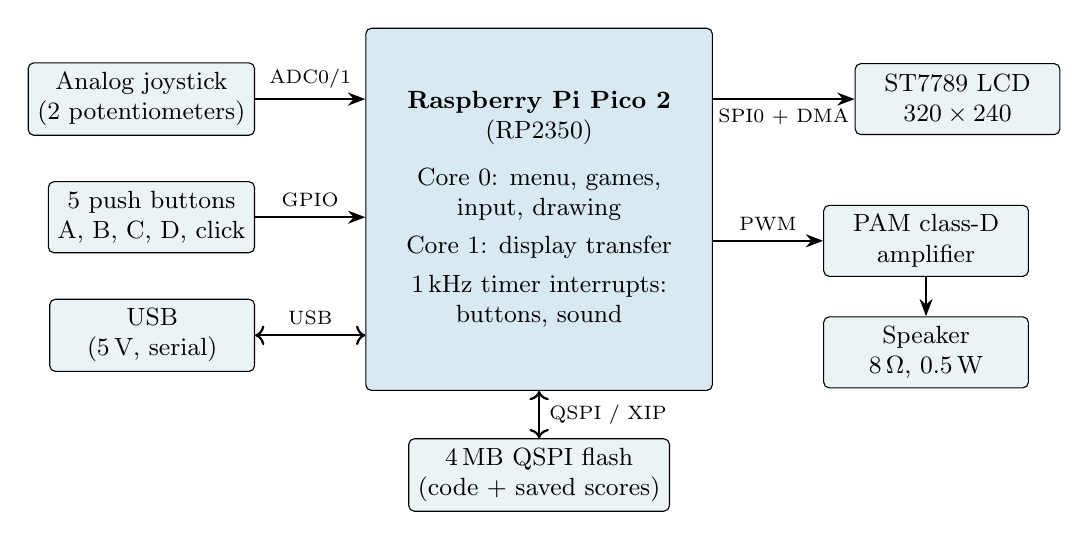
\begin{tikzpicture}[node distance=7mm and 14mm]
  \node[blk, minimum width=44mm, minimum height=46mm, fill=accent!15] (pico)
       {\textbf{Raspberry Pi Pico 2}\\(RP2350)\\[2mm]
        Core 0: menu, games,\\input, drawing\\[1mm]
        Core 1: display transfer\\[1mm]
        1\,kHz timer interrupts:\\buttons, sound};
  \node[blk, left=of pico, yshift=14mm] (joy) {Analog joystick\\(2 potentiometers)};
  \node[blk, left=of pico, yshift=-1mm] (btn) {5 push buttons\\A, B, C, D, click};
  \node[blk, left=of pico, yshift=-16mm] (usb) {USB\\(5\,V, serial)};
  \node[blk, right=18mm of pico, yshift=14mm] (lcd) {ST7789 LCD\\$320\times240$};
  \node[blk, right=of pico, yshift=-4mm] (amp) {PAM class-D\\amplifier};
  \node[blk, below=5mm of amp] (spk) {Speaker\\8\,$\Omega$, 0.5\,W};
  \node[blk, below=6mm of pico] (flash) {4\,MB QSPI flash\\(code + saved scores)};

  \draw[arr] (joy) -- node[above, font=\scriptsize]{ADC0/1} (joy -| pico.west);
  \draw[arr] (btn) -- node[above, font=\scriptsize]{GPIO} (btn -| pico.west);
  \draw[arr, <->] (usb) -- node[above, font=\scriptsize]{USB} (usb -| pico.west);
  \draw[arr] (lcd -| pico.east) -- node[below, font=\scriptsize]{SPI0 + DMA} (lcd);
  \draw[arr] (amp -| pico.east) -- node[above, font=\scriptsize]{PWM} (amp);
  \draw[arr] (amp) -- (spk);
  \draw[arr, <->] (pico) -- node[right, font=\scriptsize]{QSPI / XIP} (flash);
\end{tikzpicture}
\caption{System block diagram.}\label{fig:block}
\end{figure}

\subsection{Bill of materials}
\begin{table}[H]
\centering
\caption{Bill of materials.}
\begin{tabular}{lcl}
\toprule
\textbf{Item} & \textbf{Qty} & \textbf{Notes} \\
\midrule
Raspberry Pi Pico 2 (RP2350) & 1 & 520\,KB SRAM, 4\,MB flash \\
ST7789 SPI colour LCD module & 1 & Panel $240\times320$, used in landscape \\
Joystick shield & 1 & 2-axis analog stick with push switch, buttons A--D \\
PAM8302 class-D amplifier & 1 & Mono, powered from 3.3\,V, shutdown pin \\
Speaker & 1 & 8\,$\Omega$, 0.5\,W \\
Breadboard and jumper wires & -- & \\
USB cable & 1 & Power and data \\
\bottomrule
\end{tabular}
\end{table}

% ==========================================================
\section{Hardware}\label{sec:hardware}
% ==========================================================

\subsection{Raspberry Pi Pico 2 and the RP2350}\label{sec:pico}
The Pico~2 is a small board built around the RP2350 microcontroller.
Table~\ref{tab:rp2350} lists the parts of the chip this project relies on.

\begin{table}[H]
\centering
\caption{RP2350 features and how the project uses them.}\label{tab:rp2350}
\begin{tabularx}{\linewidth}{lX}
\toprule
\textbf{Feature} & \textbf{Detail and use} \\
\midrule
CPU & Two Arm Cortex-M33 cores at \unit{150}{MHz}, each with a single-precision floating-point unit (FPU). Core~0 runs the game; core~1 runs the display task. \\
SRAM & \unit{520}{KB}: eight striped \unit{64}{KB} banks plus two \unit{4}{KB} ``scratch'' banks used for the core stacks. Holds both framebuffers. \\
Flash & \unit{4}{MB} external QSPI flash. Code runs directly from it (execute-in-place, XIP) through a \unit{16}{KB} cache. The last \unit{4}{KB} stores best scores. \\
Clocks & One \unit{12}{MHz} crystal; phase-locked loops (PLLs) generate \unit{150}{MHz} (system) and \unit{48}{MHz} (USB, ADC). \\
SIO & Single-cycle I/O block private to each core: fast GPIO, inter-core FIFOs, event signals. \\
Peripherals used & SPI0, 1 DMA channel, ADC (2 inputs), PWM slice 7, timer alarms, USB device, flash interface. \\
\bottomrule
\end{tabularx}
\end{table}


\subsubsection{Clock tree and CPU frequency}\label{sec:clocks}
Every clock is derived from a \unit{12}{MHz} quartz crystal. The system PLL
multiplies it up to a \unit{1500}{MHz} internal oscillator (the VCO) and two
post-dividers bring it down to \unit{150}{MHz}:
\[
  f_{\text{sys}} = \frac{\unit{12}{MHz}\times 125}{5 \times 2} = \unit{150}{MHz}.
\]

\begin{figure}[H]
\centering
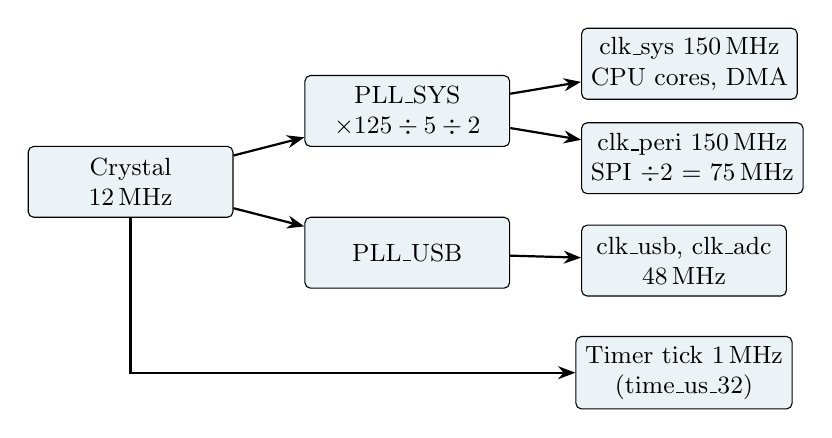
\begin{tikzpicture}[node distance=5mm and 9mm, every node/.style={font=\small}]
  \node[blk] (xosc) {Crystal\\12\,MHz};
  \node[blk, right=of xosc, yshift=9mm] (pllsys) {PLL\_SYS\\$\times125\div5\div2$};
  \node[blk, right=of xosc, yshift=-9mm] (pllusb) {PLL\_USB};
  \node[blk, right=of pllsys, yshift=6mm] (sys) {clk\_sys 150\,MHz\\CPU cores, DMA};
  \node[blk, right=of pllsys, yshift=-6mm] (peri) {clk\_peri 150\,MHz\\SPI $\div2$ = 75\,MHz};
  \node[blk, right=of pllusb, yshift=-1mm] (usb) {clk\_usb, clk\_adc\\48\,MHz};
  \node[blk, below=of usb] (ref) {Timer tick 1\,MHz\\(time\_us\_32)};
  \draw[arr] (xosc) -- (pllsys);
  \draw[arr] (xosc) -- (pllusb);
  \draw[arr] (pllsys) -- (sys);
  \draw[arr] (pllsys) -- (peri);
  \draw[arr] (pllusb) -- (usb);
  \draw[arr] (xosc.south) |- (ref);
\end{tikzpicture}
\caption{Clock tree as used by the project.}\label{fig:clocks}
\end{figure}

\begin{table}[H]
\centering
\caption{Clock frequencies.}\label{tab:clocks}
\begin{tabular}{lccl}
\toprule
\textbf{Clock} & \textbf{Normal} & \textbf{Sleep} & \textbf{Used for} \\
\midrule
clk\_sys & 150\,MHz & 48\,MHz & Both CPU cores, DMA, memory bus \\
clk\_peri & 150\,MHz & -- & SPI (divided by 2 to 75\,MHz) \\
clk\_adc & 48\,MHz & 48\,MHz & ADC (96 cycles per conversion) \\
clk\_usb & 48\,MHz & 48\,MHz & USB serial \\
Timer tick & 1\,MHz & 1\,MHz & \texttt{time\_us\_32()}, all periodic interrupts \\
\bottomrule
\end{tabular}
\end{table}

\noindent The \texttt{benchmark\_test} program checks every clock with the
RP2350's hardware frequency counter, which counts each clock against the
\unit{12}{MHz} crystal. All measured values match the configured ones:
clk\_sys = \unit{150\,000}{kHz}, clk\_peri = \unit{150\,000}{kHz},
clk\_adc = clk\_usb = \unit{48\,000}{kHz}, and clk\_ref = \unit{12\,001}{kHz}
(the counter's $\pm1$\,kHz resolution, 0.008\,\%).

\subsubsection{Memory hierarchy}\label{sec:memhier}
\begin{table}[H]
\centering
\caption{Memory hierarchy from fastest to slowest.}\label{tab:hier}
\begin{tabularx}{\linewidth}{lllX}
\toprule
\textbf{Level} & \textbf{Size} & \textbf{Access time} & \textbf{Holds in this project} \\
\midrule
CPU registers & 16 + 32 FPU & 0 extra cycles & Values being computed \\
SIO (per core) & -- & 1 cycle (6.7\,ns) & GPIO reads/writes (CS, DC, buttons) \\
SRAM & 520\,KB & 1 cycle if no bank conflict & Framebuffers, game state, stacks \\
XIP cache & 16\,KB & $\approx$1 cycle on a hit & Recently executed code \\
External flash & 4\,MB & tens of cycles on a cache miss & Program, constant data, saved scores \\
Display GRAM & 1 frame & 19.5\,ms per full frame & The image being shown \\
\bottomrule
\end{tabularx}
\end{table}

\begin{keypoint}
The Cortex-M33 cores in the RP2350 have no data cache, so both cores and the
DMA always see the same RAM contents. Correct sharing therefore only needs
\texttt{volatile} variables and memory barriers, not cache maintenance.
\end{keypoint}

\paragraph{SRAM banking.} The eight main banks are interleaved word by word, so
consecutive 4-byte words fall in different banks. A framebuffer is therefore
spread across all banks, and core~0 writing the back buffer rarely collides
with the DMA reading the front buffer in the same cycle. The core stacks live in
the two small scratch banks, so stack traffic never competes with frame data.

% ----------------------------------------------------------
\subsection{Display: ST7789 over SPI}\label{sec:display}
% ----------------------------------------------------------
The display is a TFT LCD module driven by an ST7789 controller. The controller
holds the image in its own memory (GRAM) and refreshes the panel from it, so the
picture stays on screen between transfers. The Pico writes to it over SPI; the
display never sends data back.

\subsubsection{Signals}
\begin{table}[H]
\centering
\caption{Display signals.}\label{tab:lcdsig}
\begin{tabularx}{\linewidth}{llX}
\toprule
\textbf{Signal} & \textbf{Pin} & \textbf{Function} \\
\midrule
SCK & GP18 & SPI clock. One pulse per bit; driven by the SPI hardware. \\
MOSI (SDA) & GP19 & SPI data, most significant bit first. \\
CS & GP17 & Chip select, active low. Frames each transaction; driven by software. \\
DC & GP16 & Data/command: 0 = command byte, 1 = parameter or pixel data. \\
RST & GP20 & Hardware reset, active low. \\
VCC, BL & 3V3 & Logic supply and backlight LEDs. BL is tied to 3.3\,V, so the backlight is always on. \\
\bottomrule
\end{tabularx}
\end{table}

\noindent SPI runs in mode~0: the clock idles low, the Pico changes the data bit
while the clock is low, and the display samples it on the rising edge. Eight
clock pulses carry one byte.

\subsubsection{Initialisation and commands}
After a hardware reset pulse (RST low for \unit{10}{ms}, then \unit{120}{ms} to
restart), the driver sends the commands in Table~\ref{tab:cmds}.

\begin{table}[H]
\centering
\caption{ST7789 commands used.}\label{tab:cmds}
\begin{tabular}{lll}
\toprule
\textbf{Code} & \textbf{Name} & \textbf{Purpose} \\
\midrule
\texttt{0x01} & SWRESET & Software reset \\
\texttt{0x11} & SLPOUT & Leave sleep mode (wait 120\,ms afterwards) \\
\texttt{0x3A} + \texttt{0x55} & COLMOD & 16 bits per pixel (RGB565) \\
\texttt{0x36} + \texttt{0x60} & MADCTL & Memory access order: landscape (MX + MV bits) \\
\texttt{0x20} & INVOFF & Colour inversion off \\
\texttt{0x13} & NORON & Normal display mode \\
\texttt{0x29} & DISPON & Display on \\
\texttt{0x2A}/\texttt{0x2B} & CASET/RASET & Set the column/row window \\
\texttt{0x2C} & RAMWR & Pixel data follows \\
\texttt{0x28}/\texttt{0x10} & DISPOFF/SLPIN & Display off / sleep (used by sleep mode) \\
\bottomrule
\end{tabular}
\end{table}

\paragraph{Rotation.} The panel is physically $240\times320$ (portrait). MADCTL
value \texttt{0x60} sets bit MV, which swaps rows and columns, and bit MX, which
mirrors horizontally to undo the reflection the swap introduces. The display
then behaves as $320\times240$, and the drawing code simply uses
\texttt{SCREEN\_WIDTH}~=~320 and \texttt{SCREEN\_HEIGHT}~=~240. If the image
appears upside down, \texttt{0xA0} gives the other landscape orientation.

\subsubsection{SPI speed: maximum vs.\ operating}\label{sec:spispeed}
The SPI hardware divides the \unit{150}{MHz} peripheral clock by an even
prescaler (at least 2) and a post-divider:
\[
  f_{\text{SCK}} = \frac{f_{\text{peri}}}{\text{prescale}\times\text{postdiv}},
  \qquad \text{prescale} \in \{2,4,\dots,254\},\ \text{postdiv}\in\{1,\dots,256\}.
\]
The code requests \unit{80}{MHz}. The SDK chooses the fastest rate not above the
request, $150/(2\times1) = \unit{75}{MHz}$.

\begin{table}[H]
\centering
\caption{SPI speeds.}\label{tab:spi}
\begin{tabular}{lr}
\toprule
\textbf{Quantity} & \textbf{Value} \\
\midrule
Requested (\texttt{SPI\_BAUDRATE}) & 80\,MHz \\
RP2350 maximum ($f_{\text{peri}}/2$) & 75\,MHz \\
Operating clock (chosen by the SDK) & 75\,MHz \\
ST7789 datasheet limit (16\,ns min.\ write cycle) & 62.5\,MHz \\
Measured effective throughput & 63.0\,Mbit/s \\
Actual rate reported by \texttt{spi\_get\_baudrate()} & 75\,MHz (confirmed) \\
\bottomrule
\end{tabular}
\end{table}

\noindent The panel runs about 20\,\% above its datasheet limit. This works
reliably on this module and gives the highest frame rate available.

\paragraph{Frame transfer time.} One frame is
$320 \times 240 \times 2 = \unit{153\,600}{bytes} = \unit{1\,228\,800}{bits}$.
\[
  t_{\text{ideal}} = \frac{1\,228\,800}{75\times10^{6}} = \unit{16.4}{ms},
  \qquad t_{\text{measured}} = \unit{19.5}{ms}.
\]
The difference comes from short gaps between bytes (the DMA feeds the SPI one
byte at a time), the window-setting commands sent before each frame, and
waiting for the last bits to leave the SPI hardware. The effective throughput is
$1\,228\,800/\unit{19.5}{ms} \approx \unit{63}{Mbit/s}$, about 84\,\% of the
clock rate. This transfer time is the hard upper limit on frame rate:
$1/\unit{19.5}{ms} \approx \unit{51}{FPS}$.

% ----------------------------------------------------------
\subsection{Input: analog joystick}\label{sec:joystick}
% ----------------------------------------------------------
The joystick contains two \unit{10}{k\Omega} potentiometers wired as voltage
dividers between 3.3\,V and ground. Moving the stick moves each wiper, giving a
voltage from 0 to 3.3\,V; at rest each sits near the middle.

\begin{itemize}
  \item X axis $\rightarrow$ GP26 (ADC input~0); Y axis $\rightarrow$ GP27 (ADC input~1).
  \item The joystick must be powered from 3.3\,V: the ADC pins must not exceed it.
  \item The push switch (joystick click) is a digital button on GP8 (Section~\ref{sec:buttons}).
\end{itemize}

\subsubsection{ADC and multiplexer}
The RP2350 has one 12-bit successive-approximation ADC shared between its
inputs through a multiplexer (mux). A conversion takes 96 cycles of the
\unit{48}{MHz} ADC clock:
\[
  t_{\text{conv}} = \frac{96}{\unit{48}{MHz}} = \unit{2}{\mu s}
  \quad\Rightarrow\quad \unit{500}{k\,samples/s}.
\]
Reading X then Y means switching the mux (\texttt{adc\_select\_input()}, a single
register write) and converting each time.

\begin{table}[H]
\centering
\caption{ADC timing.}\label{tab:adc}
\begin{tabular}{lcc}
\toprule
\textbf{Quantity} & \textbf{Expected} & \textbf{Measured} \\
\midrule
Resolution & 12 bits (0--4095), 0.8\,mV per step & -- \\
Conversion (\texttt{adc\_read}) & 2.0\,\textmu s (hardware) & 2.50\,\textmu s \\
Full \texttt{joystick\_read\_x()} & $\approx$2--3\,\textmu s & 3.33\,\textmu s \\
\bottomrule
\end{tabular}
\end{table}

\noindent\textbf{Interpretation.}
\begin{itemize}
  \item \textbf{Conversion:} the hardware takes \unit{2.0}{\mu s}; the measured
        \unit{2.50}{\mu s} adds about \unit{0.5}{\mu s} of software: starting
        the conversion, polling the ``ready'' flag and reading the result over the
        peripheral bus, where each register access costs several cycles.
        Polling one sample at a time therefore gives 399\,k samples/s; the full
        500\,k samples/s would need the ADC's free-running mode with DMA.
  \item \textbf{Cost per frame:} \texttt{joystick\_read\_x()} (select, convert,
        floating-point normalisation) takes \unit{3.33}{\mu s}; both axes take
        about \unit{6.7}{\mu s}, 0.03\,\% of a \unit{19.5}{ms} frame.
\end{itemize}

\subsubsection{Calibration and normalisation}
The measured raw values of this joystick are listed below. The X centre is
noticeably off the ideal 2048 and its maximum never reaches 4095.

\begin{center}
\begin{tabular}{lccc}
\toprule
& \textbf{Min} & \textbf{Centre} & \textbf{Max} \\
\midrule
X & 0 & 1769 & 3747 \\
Y & 6 & 2073 & 4095 \\
\bottomrule
\end{tabular}
\end{center}

\noindent Each side of the centre is scaled separately (piecewise-linear), so
both extremes reach exactly $\pm1$:
\[
  r = \begin{cases}
    \dfrac{v - c}{c - v_{\min}} & v < c \\[2ex]
    \dfrac{v - c}{v_{\max} - c} & v \ge c
  \end{cases}
  \qquad\text{then clamp to } [-1, 1],\quad |r| < 0.2 \Rightarrow r = 0.
\]
The final step is a 20\,\% \emph{dead zone}: small readings caused by electrical
noise, or by the spring not returning exactly to centre, become exactly zero so
the ship does not drift. Example: X raw 885 gives $(885-1769)/1769 = -0.50$.

\paragraph{How the games use it.} Space Shooter uses the value proportionally
(half a push gives half the acceleration). Snake converts it to four directions
with a 0.6 threshold on the dominant axis. The menu uses hysteresis: a step
when $|x| > 0.6$, re-armed only after $|x| < 0.3$, so one push moves exactly one
card. Screen $y$ grows downwards, so the games use $-y$.

% ----------------------------------------------------------
\subsection{Input: push buttons}\label{sec:buttons}
% ----------------------------------------------------------
Each button connects a GPIO pin to ground. The pin's internal pull-up resistor
(about \unit{50}{k\Omega}) holds it at logic 1 when released; pressing pulls it
to 0. The buttons are therefore \emph{active-low}, and no external resistors are
needed.

\begin{center}
\begin{tabular}{lcl}
\toprule
\textbf{Button} & \textbf{Pin} & \textbf{Main use} \\
\midrule
A & GP2 & Fire up; hold 3\,s on the menu to reset scores \\
B & GP3 & Fire right; next game on the menu \\
C & GP4 & Shield; FPS overlay toggle on the menu \\
D & GP5 & Fire left; previous game; back to menu \\
Joystick click & GP8 & Start, pause/resume; hold 2\,s on the menu to sleep \\
\bottomrule
\end{tabular}
\end{center}

% ----------------------------------------------------------
\subsection{Audio: PWM, PAM amplifier and speaker}\label{sec:audiohw}
% ----------------------------------------------------------
\begin{figure}[H]
\centering
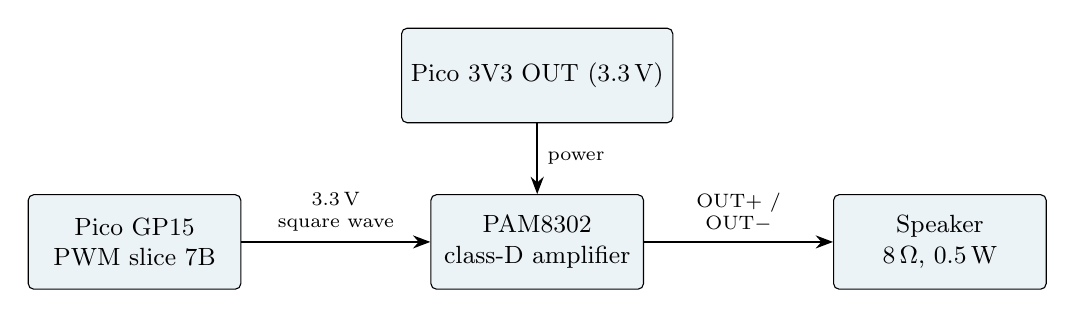
\begin{tikzpicture}[node distance=24mm,
                    blk/.append style={minimum width=27mm, minimum height=12mm}]
  \node[blk] (pwm) {Pico GP15\\PWM slice 7B};
  \node[blk, right=of pwm] (amp) {PAM8302\\class-D amplifier};
  \node[blk, right=of amp] (spk) {Speaker\\8\,$\Omega$, 0.5\,W};
  \node[blk, above=9mm of amp] (vbus) {Pico 3V3 OUT (3.3\,V)};
  \draw[arr] (pwm) -- node[above, font=\scriptsize, align=center]{3.3\,V\\square wave} (amp);
  \draw[arr] (amp) -- node[above, font=\scriptsize, align=center]{OUT$+$ /\\OUT$-$} (spk);
  \draw[arr] (vbus) -- node[right, font=\scriptsize]{power} (amp);
\end{tikzpicture}
\caption{Audio signal chain.}
\end{figure}

\paragraph{Why an amplifier.} A speaker has an impedance of a few ohms. At
3.3\,V an \unit{8}{\Omega} speaker would try to draw about \unit{0.4}{A}, far
above the few milliamps a GPIO pin can supply. The amplifier takes the weak
logic-level signal and drives the speaker with power taken from the Pico's 3.3\,V supply.

\paragraph{Class-D operation.} A class-D amplifier switches its output
transistors fully on or off at several hundred kilohertz, itself a form of PWM.
The speaker coil cannot follow such fast switching and averages it, reproducing
only the audio. Because the transistors are always fully on or fully off, very
little power is lost as heat (about 85--90\,\% efficiency), so no heatsink is
needed.

\paragraph{The PAM8302 module.} The PAM8302 is a mono class-D amplifier that
runs from 2.0--5.5\,V; here it is powered from the Pico's 3V3 OUT pin. Its
input is differential (A$+$/A$-$): GP15 drives A$+$ and A$-$ goes to ground.
The output power is limited by the supply voltage. With a bridge-tied output the
peak voltage across the speaker is about $V_{DD}$, so
\[
  P_{\max} \approx \frac{V_{DD}^2}{2R} = \frac{(3.3)^2}{2 \times 8} \approx \unit{0.68}{W}
\]
in theory, and roughly 0.5\,W in practice after losses. This matches the
0.5\,W speaker, so it cannot be badly overdriven. (At 5\,V the same module could
deliver about 1.5\,W into 8\,$\Omega$.) Loud sounds can draw current peaks of
around 0.2\,A from the 3.3\,V rail, which also feeds the display, so a decoupling
capacitor (e.g.\ 100\,\textmu F) across the amplifier's supply pins helps keep
the rail steady. The module also has a shutdown (SD) pin,
which could switch the amplifier off during sleep (Section~\ref{sec:power}).

\paragraph{Bridge-tied output.} The PAM output drives both speaker wires in
opposite directions, doubling the voltage swing. The speaker's negative wire
must therefore go to OUT$-$, never to ground.

\paragraph{Ground.} The Pico and the amplifier share one ground; otherwise the
input signal has no common reference.

% ----------------------------------------------------------
\subsection{Power distribution}\label{sec:powerhw}
% ----------------------------------------------------------
\begin{figure}[H]
\centering
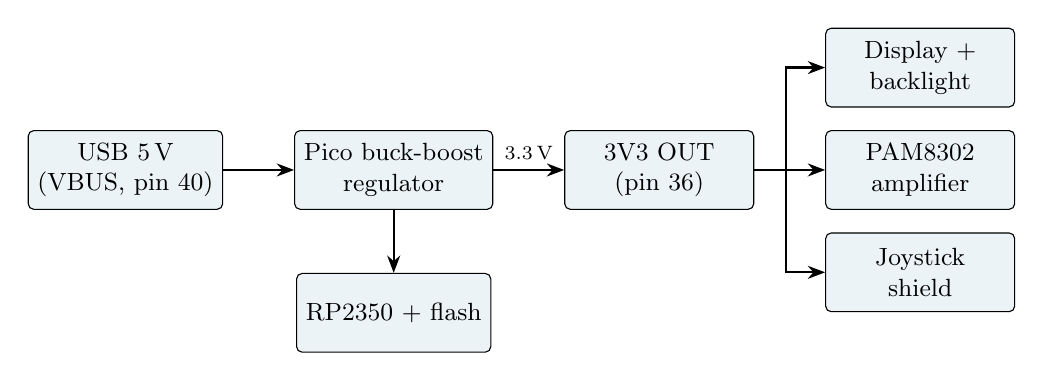
\begin{tikzpicture}[node distance=8mm and 9mm,
                    blk/.append style={minimum width=24mm, minimum height=10mm}]
  \node[blk] (usb) {USB 5\,V\\(VBUS, pin 40)};
  \node[blk, right=of usb] (reg) {Pico buck-boost\\regulator};
  \node[blk, right=of reg] (v33) {3V3 OUT\\(pin 36)};
  \node[blk, right=of v33, yshift=13mm] (lcd) {Display +\\backlight};
  \node[blk, right=of v33] (amp) {PAM8302\\amplifier};
  \node[blk, right=of v33, yshift=-13mm] (js) {Joystick\\shield};
  \node[blk, below=of reg] (chip) {RP2350 + flash};
  \draw[arr] (usb) -- (reg);
  \draw[arr] (reg) -- node[above, font=\scriptsize]{3.3\,V} (v33);
  \draw[arr] (reg) -- (chip);
  \draw[arr] (v33.east) -- ++(4mm,0) |- (lcd.west);
  \draw[arr] (v33.east) -- (amp.west);
  \draw[arr] (v33.east) -- ++(4mm,0) |- (js.west);
\end{tikzpicture}
\caption{Power distribution. All grounds are connected together.}
\end{figure}

\noindent The Pico's regulator produces a steady 3.3\,V for the RP2350, its
flash, and the 3V3 OUT pin; inside the chip a further regulator makes the core
supply of about 1.1\,V. Every external module (display, amplifier and joystick)
is powered from 3V3 OUT, so the whole handheld runs on one 3.3\,V rail. The Pico
documentation recommends drawing no more than about 300\,mA from 3V3 OUT; the
display and backlight take a few tens of milliamps and the amplifier draws its
peaks only while a sound plays, so this budget is respected.

% ----------------------------------------------------------
\subsection{Pin assignment}\label{sec:pins}
% ----------------------------------------------------------
\small\begin{longtable}{cclp{2.2cm}p{3.6cm}}
\caption{Complete pin assignment.}\label{tab:pins}\\
\toprule
\textbf{Pin} & \textbf{GPIO} & \textbf{Connected to} & \textbf{Peripheral} & \textbf{Notes} \\
\midrule\endfirsthead
\toprule
\textbf{Pin} & \textbf{GPIO} & \textbf{Connected to} & \textbf{Peripheral} & \textbf{Notes} \\
\midrule\endhead
4 & GP2 & Button A & GPIO in & Pull-up, active low \\
5 & GP3 & Button B & GPIO in & Pull-up, active low \\
6 & GP4 & Button C & GPIO in & Pull-up, active low \\
7 & GP5 & Button D & GPIO in & Pull-up, active low \\
11 & GP8 & Joystick click & GPIO in & Pull-up, active low \\
20 & GP15 & Amplifier input & PWM 7B & Amp input ground to Pico GND \\
21 & GP16 & Display DC & GPIO out & \\
22 & GP17 & Display CS & GPIO out & \\
24 & GP18 & Display SCK & SPI0 SCK & 75\,MHz \\
25 & GP19 & Display MOSI/SDA & SPI0 TX & \\
26 & GP20 & Display RST & GPIO out & \\
31 & GP26 & Joystick X & ADC0 & Max 3.3\,V \\
32 & GP27 & Joystick Y & ADC1 & Max 3.3\,V \\
36 & 3V3 & VCC of all modules & Power & Display, BL, joystick, amplifier \\
38 etc. & GND & All grounds & Ground & Common ground \\
\bottomrule
\end{longtable}\normalsize

% ==========================================================
\section{Software Architecture}\label{sec:software}
% ==========================================================

\subsection{Modules}
The firmware is written in C on the Raspberry Pi Pico SDK~2.3.1. Each hardware
function lives in its own module with a small header. Table~\ref{tab:modules}
lists every file; the sizes are the code and constant data each module
contributes to flash, and the RAM it reserves.

\small\begin{longtable}{p{3.3cm}p{7.3cm}rr}
\caption{Source modules (sizes from the compiled object files).}\label{tab:modules}\\
\toprule
\textbf{File} & \textbf{Responsibility} & \textbf{Flash (B)} & \textbf{RAM (B)} \\
\midrule\endfirsthead
\toprule
\textbf{File} & \textbf{Responsibility} & \textbf{Flash (B)} & \textbf{RAM (B)} \\
\midrule\endhead
\file{handheld.c} & Entry point: hardware init, load scores, start menu & 52 & 0 \\
\file{menu.c} & Game-select menu, FPS toggle, score reset, hold-to-sleep & 1\,997 & 4 \\
\file{space\_shooter.c} & Space Shooter game & 11\,676 & 3\,383 \\
\file{snake.c} & Snake game & 2\,784 & 1\,384 \\
\file{display/}\allowbreak\file{display.c} & ST7789 driver, framebuffers, DMA, core~1 task, drawing, font, FPS statistics & 5\,077 & 307\,279 \\
\file{input/buttons.c} & 1\,kHz sampling, debounce, press latching & 640 & 48 \\
\file{input/joystick.c} & ADC reading, calibration, dead zone & 552 & 0 \\
\file{sound/sound.c} & Non-blocking PWM sound effects & 820 & 50 \\
\file{save/save.c} & Best scores in flash & 704 & 284 \\
\file{power/power.c} & Sleep and wake & 570 & 4 \\
\file{ui/ui.c} & Shared drawing helpers, colours, pause box & 1\,311 & 0 \\
\midrule
\textbf{Application total} & & \textbf{26\,183} & \textbf{312\,436} \\
Pico SDK + C library & USB stack, printf, maths, start-up, multicore, flash & 39\,013 & 5\,292 \\
\midrule
\textbf{Firmware total} & & \textbf{65\,196} & \textbf{317\,728} \\
\bottomrule
\end{longtable}\normalsize

\noindent The test programs in \file{test/} (\texttt{display\_test},
\texttt{buttons\_test}, \texttt{joystick\_test}, \texttt{sound\_test} and
\texttt{benchmark\_test}) reuse the same modules.

\subsection{Execution model}
Three kinds of execution context run at the same time:

\begin{table}[H]
\centering
\caption{Execution contexts.}\label{tab:contexts}
\begin{tabularx}{\linewidth}{llX}
\toprule
\textbf{Context} & \textbf{Where} & \textbf{Work} \\
\midrule
Main loop & Core 0 & Menu or game: read input snapshot, update logic, draw the frame, call \texttt{display\_show()} \\
Display task & Core 1 & Wait for a finished frame, set the window, run the DMA transfer, signal completion \\
Button interrupt & Core 0, 1\,kHz & Sample 5 pins, debounce, latch presses \\
Sound interrupt & Core 0, 1\,kHz & Advance the current sound effect, update the PWM frequency \\
\bottomrule
\end{tabularx}
\end{table}

\subsection{Boot sequence}
\begin{enumerate}
  \item The boot ROM checks BOOTSEL, finds the program's image definition in flash and starts it on core~0. Core~1 waits in the boot ROM.
  \item The C runtime copies initialised data to RAM, zeroes \texttt{.bss} (including the framebuffers), sets the clocks to 150\,MHz and calls \texttt{main()}.
  \item \texttt{main()} starts USB serial, then initialises the display (which launches core~1), buttons, joystick and sound.
  \item Saved best scores are loaded from flash and the random generator is seeded from the timer.
  \item \texttt{menu\_run()} starts and never returns.
\end{enumerate}

% ==========================================================
\section{Rendering Pipeline}\label{sec:render}
% ==========================================================

\subsection{Framebuffer and pixel format}
Every frame is drawn into a RAM array of $320\times240$ pixels, then sent to the
display in one transfer. The screen never shows a half-drawn picture, so there is
no flicker.

Each pixel is 16 bits in RGB565 format: 5 bits red, 6 bits green, 5 bits blue.
Green gets the extra bit because the eye is most sensitive to it. A 24-bit colour
is converted with
\[
  \text{RGB565}(r,g,b) = \big((r \,\&\, \texttt{0xF8}) \ll 8\big) \;|\;
                         \big((g \,\&\, \texttt{0xFC}) \ll 3\big) \;|\; (b \gg 3).
\]
The RP2350 stores 16-bit values low byte first, but the ST7789 expects the high
byte first, so each pixel is byte-swapped when it is written. The DMA can then
copy the buffer to SPI unchanged.

\subsection{Sprites and drawing primitives}
The game objects are \emph{procedural sprites}: they are drawn from geometric
primitives at run time rather than copied from stored images. Small fixed
graphics (the 5$\times$7 font and the heart icon) are stored as bitmaps.

\begin{table}[H]
\centering
\caption{Drawing primitives.}\label{tab:prims}
\begin{tabularx}{\linewidth}{lX}
\toprule
\textbf{Primitive} & \textbf{Algorithm} \\
\midrule
Line & Bresenham's algorithm: integer-only stepping along the major axis \\
Filled rectangle & Clipped to the screen, then a row-by-row fill \\
Circle outline & Midpoint circle algorithm, drawing 8 symmetric points per step \\
Filled circle & One horizontal span per row, half-width $\sqrt{r^2-d_y^2}$ \\
Filled triangle & Vertices sorted by $y$; each scanline filled between the two interpolated edges \\
Text & 5$\times$7 bitmap font (39 glyphs), scaled by drawing each set bit as a square \\
\bottomrule
\end{tabularx}
\end{table}

\noindent Examples: the ship is three filled triangles (two wings and the hull),
a filled circle (cockpit) and a flickering triangular flame. An asteroid is a
filled circle plus an 8-vertex jagged outline rotated by $(\cos\theta,
\sin\theta)$ each frame, plus two crater circles. The cost of each primitive is
measured by \texttt{benchmark\_test} (Section~\ref{sec:profile}).

\subsection{DMA transfer}
One DMA channel is configured to copy $153\,600$ bytes from the framebuffer to
the SPI data register:
\begin{itemize}
  \item transfer size 8 bits; read address increments, write address fixed;
  \item paced by the SPI transmit request signal (DREQ), so the DMA writes only
        when the SPI has room;
  \item before the DMA starts, the CPU sends CASET, RASET and RAMWR with DC
        toggled, then holds DC~=~1 and CS~=~0 for the whole burst.
\end{itemize}
The DMA moves the data with no CPU involvement. Some code must still wait for
it to finish before raising CS and reusing the buffer, and that is the job
given to core~1.

\subsection{Dual-core double buffering}\label{sec:dualcore}
With one framebuffer, core~0 must wait \unit{19.5}{ms} for every transfer,
because it cannot draw into memory that is being sent. With two framebuffers,
core~0 draws the next frame while core~1 sends the previous one
(Figure~\ref{fig:pipeline}).

\begin{figure}[H]
\centering
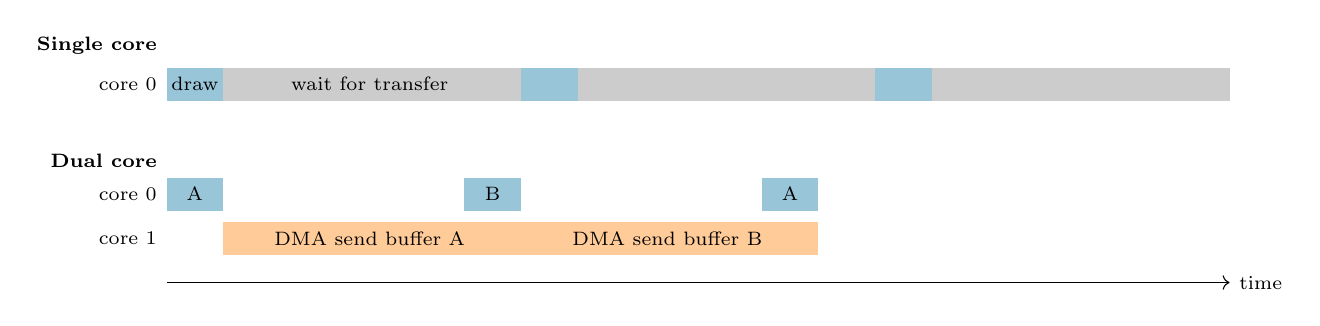
\begin{tikzpicture}[x=6mm, y=7mm, every node/.style={font=\scriptsize}]
  % single core
  \node[anchor=east] at (0,3) {\textbf{Single core}};
  \node[anchor=east] at (0,2.3) {core 0};
  \foreach \s in {0,7.5,15} {
     \fill[accent!40] (\s,2) rectangle (\s+1.2,2.6);
     \fill[gray!40] (\s+1.2,2) rectangle (\s+7.5,2.6);
  }
  \node at (0.6,2.3) {draw}; \node at (4.3,2.3) {wait for transfer};
  % dual core
  \node[anchor=east] at (0,0.9) {\textbf{Dual core}};
  \node[anchor=east] at (0,0.3) {core 0};
  \node[anchor=east] at (0,-0.5) {core 1};
  \foreach \i/\b in {0/A,1/B,2/A} {
     \fill[accent!40] (\i*6.3,0) rectangle (\i*6.3+1.2,0.6);
     \node at (\i*6.3+0.6,0.3) {\b};
  }
  \foreach \i/\b in {0/A,1/B} {
     \fill[orange!40] (1.2+\i*6.3,-0.8) rectangle (1.2+\i*6.3+6.3,-0.2);
     \node at (1.2+\i*6.3+3.1,-0.5) {DMA send buffer \b};
  }
  \draw[->] (0,-1.3) -- (22.5,-1.3) node[right]{time};
\end{tikzpicture}
\caption{Frame pipeline. Core~0 draws in about 3\,ms; a transfer takes 19.5\,ms.
In dual-core mode the transfer overlaps the drawing of the next frame.}\label{fig:pipeline}
\end{figure}

\paragraph{Hand-off protocol.} The two cores share three variables:
\texttt{transfer\_busy}, \texttt{transfer\_index} and
\texttt{core1\_transfer\_us}. Core~0, in \texttt{display\_show()}:

\begin{lstlisting}
while (transfer_busy) __wfe();       // wait until core 1 finished the last frame
__dmb();
transfer_index = back_index;         // hand over the frame just drawn
__dmb();
transfer_busy = true;
__sev();                             // wake core 1
back_index ^= 1;                     // draw the next frame in the other buffer
framebuffer = framebuffers[back_index];
\end{lstlisting}

\noindent Core~1 runs forever:

\begin{lstlisting}
flash_safe_execute_core_init();      // allow core 0 to pause us during flash writes
while (true) {
    while (!transfer_busy) __wfe();  // sleep until there is a frame
    __dmb();
    transfer_frame(framebuffers[transfer_index]);   // window + DMA + wait
    __dmb();
    transfer_busy = false;
    __sev();                         // wake core 0 if it is waiting
}
\end{lstlisting}

\begin{itemize}
  \item \texttt{volatile} forces each read of a shared variable to come from
        memory instead of a stale register copy.
  \item \texttt{\_\_dmb()} (data memory barrier) makes sure the buffer index is
        written before \texttt{transfer\_busy} becomes visible to the other core.
  \item \texttt{\_\_wfe()} (wait for event) puts a core to sleep until the other
        core executes \texttt{\_\_sev()} (send event). Each core has a one-bit
        event flag that remembers a pending event, so a wake-up sent just before
        the other core goes to sleep is never lost.
\end{itemize}

\paragraph{Why this split.} The transfer is the largest cost (\unit{19.5}{ms}
against \unit{3}{ms} of drawing) and is completely independent of game logic once
a frame is finished, so moving it to core~1 gives the largest gain. The two cores
share only three small variables, so no locks are needed in the game code, and the
games themselves did not change: they still just call \texttt{display\_show()}.
Splitting the drawing itself between the cores would gain little, since drawing
takes only 3\,ms. Splitting game logic from drawing would require locking all
game state.

\paragraph{Build option.} The CMake option \texttt{HANDHELD\_DUAL\_CORE=OFF}
builds a single-core version (one buffer, blocking transfer) from the same
source, for the comparison in Section~\ref{sec:fps}.

\subsection{FPS measurement}\label{sec:fpsmethod}
\texttt{display\_show()} timestamps every frame with the \unit{1}{MHz} hardware
timer. Over each one-second window it computes:
\begin{itemize}
  \item FPS = frames / elapsed time;
  \item average and worst frame time;
  \item average DMA transfer time (measured on core~1);
  \item average time core~0 spent \emph{waiting} for the display;
  \item core~0 \emph{render} time = frame time $-$ wait time (logic + drawing).
\end{itemize}
The results are printed over USB once per second and can be shown on screen
(press C on the menu).

% ==========================================================
\section{Input Handling}\label{sec:input}
% ==========================================================

\subsection{Problems solved}
\begin{enumerate}
  \item \textbf{Contact bounce.} A mechanical contact bounces open and closed for
        1--5\,ms when pressed or released, so one press can look like several.
  \item \textbf{Missed presses.} A game reading the pins once per frame
        (every 19.5\,ms) can miss a short tap that falls between two reads.
  \item \textbf{Inconsistent reads.} Different parts of one frame reading the pin
        at different moments could disagree.
\end{enumerate}

\subsection{Design: interrupt producer, frame consumer}
A repeating timer interrupt runs every \unit{1}{ms} (polling frequency
\unit{1}{kHz}) on core~0 and performs a counter-based debounce:

\begin{lstlisting}
bool raw_down = (gpio_get(pin) == 0);            // active-low
if (raw_down == stable_down[i]) {                // agrees: nothing to do
    change_count[i] = 0;
} else if (++change_count[i] >= BUTTON_DEBOUNCE_MS) {   // 5 ms in a row
    stable_down[i] = raw_down;                   // accept the new state
    change_count[i] = 0;
    if (raw_down) pending_presses[i]++;          // latch the press
}
\end{lstlisting}

\noindent A change is accepted only after the pin has read the new value for
\unit{5}{ms} in a row; any bounce back resets the count. Every accepted press
increments a counter, so it is remembered until the game reads it.

\begin{table}[H]
\centering
\caption{Debounce example: a press with one bounce.}
\begin{tabular}{cccl}
\toprule
\textbf{ms} & \textbf{Raw pin} & \textbf{Count} & \textbf{Stable state} \\
\midrule
0 & 0 (pressed) & 1 & released \\
1 & 1 (bounce) & 0 (reset) & released \\
2 & 0 & 1 & released \\
3--5 & 0 & 2--4 & released \\
6 & 0 & 5 & \textbf{pressed}, press counter $+1$ \\
\bottomrule
\end{tabular}
\end{table}

Once per frame the game calls \texttt{buttons\_poll()}, which copies the press
counters into a per-frame snapshot and clears them. Interrupts are disabled for
these few microseconds (a \emph{critical section}), so a press arriving between
the copy and the clear cannot be lost. The game then asks:
\begin{itemize}
  \item \texttt{button\_just\_pressed(b)}: true for exactly one frame per press
        (pause, shield, menu steps, Snake turns);
  \item \texttt{button\_down(b)}: true while held (continuous firing, hold timers).
\end{itemize}
\texttt{buttons\_clear()} discards unread presses when switching screens, so the
press that leaves a game cannot also act in the menu.

\subsection{Timing figures}
\begin{table}[H]
\centering
\caption{Input timing.}\label{tab:inputtiming}
\begin{tabular}{lr}
\toprule
\textbf{Quantity} & \textbf{Value} \\
\midrule
Button polling frequency & 1\,kHz (every 1\,ms) \\
Debounce time & 5\,ms \\
Press recognised after the contact closes & 5--6\,ms \\
Shortest press accepted & 5\,ms \\
Presses remembered between frames & up to 255 per button \\
Joystick polling & once per frame per axis ($\approx$51\,Hz) \\
\bottomrule
\end{tabular}
\end{table}

\paragraph{End-to-end input latency (estimate).} From pressing a button to seeing
the result on screen:
\[
  \underbrace{5\text{--}6}_{\text{debounce}} +
  \underbrace{0\text{--}19.5}_{\text{until next poll}} +
  \underbrace{3}_{\text{logic + draw}} +
  \underbrace{19.5}_{\text{transfer}} \approx \unit{28\text{--}48}{ms}.
\]
This is below the roughly 50\,ms at which delay becomes noticeable to a player.
The display's own refresh adds up to one more panel refresh period on top. The
latency can be measured by filming the screen and a button press with a
high-speed phone camera.

% ==========================================================
\section{Audio Engine}\label{sec:audio}
% ==========================================================

\subsection{Tone generation with PWM}
A PWM slice is a 16-bit counter that counts from 0 to TOP and wraps; the output
is high while the counter is below LEVEL. With clock divider DIV:
\[
  f = \frac{f_{\text{sys}}}{\text{DIV}\times(\text{TOP}+1)},\qquad
  \text{duty} = \frac{\text{LEVEL}}{\text{TOP}+1}.
\]
TOP cannot exceed 65\,535, so without a divider the lowest note would be
$150\,\text{MHz}/65\,536 \approx \unit{2.3}{kHz}$. The code chooses the
smallest divider that keeps TOP within 16 bits:
\[
  \text{DIV} = \left\lfloor\frac{f_{\text{sys}}}{65\,536\, f}\right\rfloor + 1,\qquad
  \text{TOP} = \frac{f_{\text{sys}}}{\text{DIV}\cdot f} - 1,\qquad
  \text{LEVEL} = \text{TOP}/2.
\]
Example, A4 = 440\,Hz: DIV = 6, TOP = 56\,817, LEVEL = 28\,408, giving
$150\times10^6/(6\times56\,818) = \unit{440.0}{Hz}$. The usable range is about
20\,Hz to 8\,kHz. The duty cycle is fixed at 50\,\%, which gives the strongest
fundamental tone.

Note frequencies follow equal temperament, $f = 440 \times 2^{(n-69)/12}$
(MIDI note $n$), and are stored as constants in \file{sound/notes.h}.

\subsection{Non-blocking sound effects}
The original code played tones with \texttt{sleep\_ms()}, freezing the game for
every beep. The engine now runs in a \unit{1}{kHz} timer interrupt. A sound
effect is a list of segments, each sliding its pitch linearly from a start to an
end frequency over a number of milliseconds:
\[
  f(t) = f_{\text{start}} + (f_{\text{end}} - f_{\text{start}})\,\frac{t}{T}.
\]
Explosion-like sounds add pseudo-random jitter of $\pm50\,\%$ every
millisecond, using a 16-bit linear-feedback shift register (LFSR), a very fast
pseudo-random generator. Each effect has a priority, so a frequent laser shot can
never cut off an important sound such as being hit.

\begin{longtable}{lllc}
\caption{Sound effects.}\label{tab:sfx}\\
\toprule
\textbf{Effect} & \textbf{Segments (Hz, ms)} & \textbf{Character} & \textbf{Priority} \\
\midrule\endfirsthead
\toprule
\textbf{Effect} & \textbf{Segments (Hz, ms)} & \textbf{Character} & \textbf{Priority} \\
\midrule\endhead
Shoot & 1800$\to$700, 45 & falling ``pew'' & 1 \\
Explosion & 900$\to$250, 160, noise & crunch & 2 \\
Shield blocks rock & 2000, 25; 1400, 50 & metallic ``ting'' & 2 \\
Orb pickup & 880, 45; 1319, 45; 1760, 70 & rising chime & 3 \\
Shield on & 500$\to$1800, 160 & rising sweep & 3 \\
Hit & 700$\to$250, 120 noise; 300$\to$150, 160 noise & heavy crash & 4 \\
Snake eats & 1047, 40; 1568, 60 & two-note blip & 2 \\
Snake crash & 800$\to$200, 250, noise & crunch & 4 \\
Menu move & 1300, 25 & blip & 1 \\
Menu select & 600$\to$1800, 120 & sweep & 5 \\
\bottomrule
\end{longtable}

% ==========================================================
\section{Persistent Scores in Flash}\label{sec:save}
% ==========================================================

\subsection{Flash constraints}
\begin{itemize}
  \item \textbf{Erase} works on whole \unit{4}{KB} sectors and sets every bit
        to 1. \textbf{Program} works on \unit{256}{byte} pages and can only change
        bits from 1 to 0, so data cannot be overwritten in place.
  \item Each sector survives about $10^5$ erase cycles.
  \item While flash is being erased or programmed it cannot be read, so no code
        can execute from it. Both interrupts and core~1 must be paused.
\end{itemize}

\subsection{Record format}
The last 4\,KB sector of flash (offset \texttt{0x3FF000}) is divided into 16
pages. Each save writes one 24-byte record into the next empty page.

\begin{table}[H]
\centering
\caption{Save record (24 bytes, padded to a 256-byte page with \texttt{0xFF}).}
\begin{tabular}{llll}
\toprule
\textbf{Offset} & \textbf{Field} & \textbf{Size} & \textbf{Purpose} \\
\midrule
0 & magic & 4\,B & \texttt{0x48485343} (``HHSC''): marks our data \\
4 & version & 4\,B & Record format version (1) \\
8 & sequence & 4\,B & Increases with each save; the highest is newest \\
12 & scores[0] & 4\,B & Space Shooter best \\
16 & scores[1] & 4\,B & Snake best \\
20 & checksum & 4\,B & CRC32 of bytes 0--19 \\
\bottomrule
\end{tabular}
\end{table}

\subsection{Algorithms}
\paragraph{Loading.} At start-up all 16 pages are scanned; a page counts as
valid only if its magic number, version and CRC32 all match, and the valid
record with the highest sequence number wins. A record half-written when power
was lost fails the CRC and is ignored, so the previous good record is used.

\paragraph{Saving (wear levelling).} A score is written only when it beats the
stored best. The record goes into the next page; the sector is erased only when
all 16 pages are used, or the next page is not blank. This gives 16 times fewer
erases than rewriting one fixed location:
\[
  \text{lifetime} \approx 10^5\ \text{erases} \times 16\ \text{saves per erase}
  = 1.6\times10^{6}\ \text{saves}.
\]

\paragraph{Safe writes.} The write runs inside \texttt{flash\_safe\_execute()},
which disables interrupts and parks core~1 (registered with
\texttt{flash\_safe\_execute\_core\_init()}) in RAM while flash is busy. The SDK
flash routines themselves run from RAM and flush the XIP cache afterwards.

\paragraph{Verification.} The module was tested on a PC against a simulated
flash chip: scores survived a simulated reboot; 41 saves caused only 3 sector
erases; a corrupted newest record correctly fell back to the previous one; and
nothing outside the save sector was modified.

\paragraph{Reset.} Holding A for 3\,s on the menu resets all best scores.

% ==========================================================
\section{Power Management and Sleep}\label{sec:power}
% ==========================================================

The handheld has no lid, so ``sleep on close'' is triggered from software:
\begin{itemize}
  \item holding the joystick click for 2\,s on the menu, or
  \item 60\,s without any input on a calm screen (menu, title, pause, game over;
        never during play).
\end{itemize}

\begin{figure}[H]
\centering
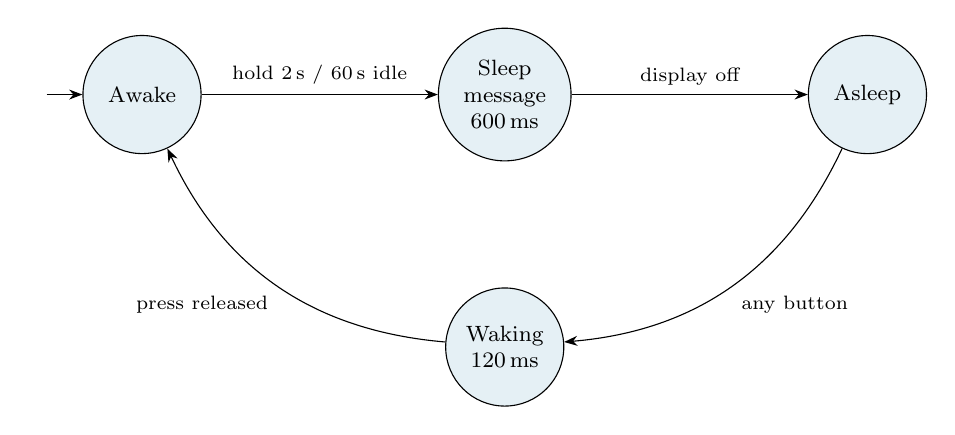
\begin{tikzpicture}[->, >=Stealth, node distance=30mm, auto]
  \node[state, initial, initial text=] (awake) {Awake};
  \node[state, right=of awake] (msg) {Sleep\\message\\600\,ms};
  \node[state, right=of msg] (asleep) {Asleep};
  \node[state, below=16mm of msg] (wake) {Waking\\120\,ms};
  \path (awake) edge node[font=\scriptsize]{hold 2\,s / 60\,s idle} (msg)
        (msg) edge node[font=\scriptsize]{display off} (asleep)
        (asleep) edge[bend left] node[font=\scriptsize]{any button} (wake)
        (wake) edge[bend left] node[font=\scriptsize]{press released} (awake);
\end{tikzpicture}
\caption{Sleep state machine.}\label{fig:sleepfsm}
\end{figure}

\begin{table}[H]
\centering
\caption{What happens on sleep and wake.}
\begin{tabularx}{\linewidth}{lX}
\toprule
\textbf{Step} & \textbf{Action} \\
\midrule
1 & Stop all sound \\
2 & Show ``SLEEPING'' for 600\,ms \\
3 & Wait for core~1 to finish any transfer, then send DISPOFF and SLPIN \\
4 & Wait until the triggering button is released \\
5 & Lower clk\_sys from 150 to 48\,MHz \\
6 & Core~0 sleeps in \texttt{\_\_wfi()} (wait for interrupt), checking the buttons each time the 1\,ms interrupt wakes it; core~1 is already idle in \texttt{\_\_wfe()} \\
7 & On a press: restore 150\,MHz, send SLPOUT, wait 120\,ms, send DISPON \\
8 & Wait for the release, discard the press, reset the FPS statistics, resume \\
\bottomrule
\end{tabularx}
\end{table}

\paragraph{Limitation.} The backlight is wired straight to 3.3\,V, so it stays
lit during sleep and cannot be dimmed. Connecting BL to a GPIO would allow it to
be switched off, which is likely the largest single saving available. The
amplifier also draws a small idle current; if the module has a shutdown pin, it
could be turned off during sleep the same way.

% ==========================================================
\section{Games and State Machines}\label{sec:games}
% ==========================================================

Every screen is implemented as a finite state machine: a variable holds the
current state, and inputs or timers cause transitions.

\subsection{Menu}
\begin{figure}[H]
\centering
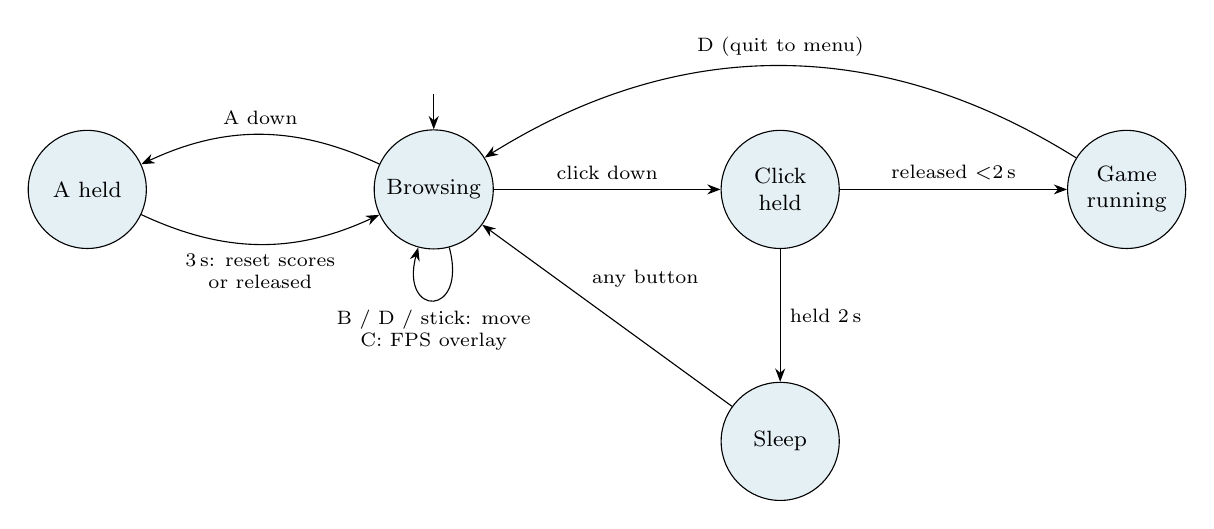
\begin{tikzpicture}[->, >=Stealth, auto, every edge quotes/.style={font=\scriptsize}]
  \node[state, initial, initial where=above, initial text=] (browse) at (0,0) {Browsing};
  \node[state] (ahold) at (-4.4,0) {A held};
  \node[state] (held)  at (4.4,0) {Click\\held};
  \node[state] (game)  at (8.8,0) {Game\\running};
  \node[state] (sleep) at (4.4,-3.2) {Sleep};
  \path (browse) edge[bend right=25] node[above, font=\scriptsize]{A down} (ahold)
        (ahold)  edge[bend right=25] node[below, font=\scriptsize, align=center]{3\,s: reset scores\\or released} (browse)
        (browse) edge node[above, font=\scriptsize]{click down} (held)
        (held)   edge node[above, font=\scriptsize]{released $<$2\,s} (game)
        (held)   edge node[right, font=\scriptsize]{held 2\,s} (sleep)
        (sleep)  edge node[pos=0.6, above right, font=\scriptsize]{any button} (browse)
        (game)   edge[bend right=32] node[above, font=\scriptsize]{D (quit to menu)} (browse)
        (browse) edge[loop below, looseness=6] node[below, font=\scriptsize, align=center]{B / D / stick: move\\C: FPS overlay} (browse);
\end{tikzpicture}
\caption{Menu state machine.}
\end{figure}

\noindent Games are listed in a table of \{name, icon function, run function,
best-score function\}; adding a game means adding one entry. Holding the click
starts the game only on release, so that a long hold can mean sleep instead.

\subsection{Space Shooter}\label{sec:shooter}
\begin{figure}[H]
\centering
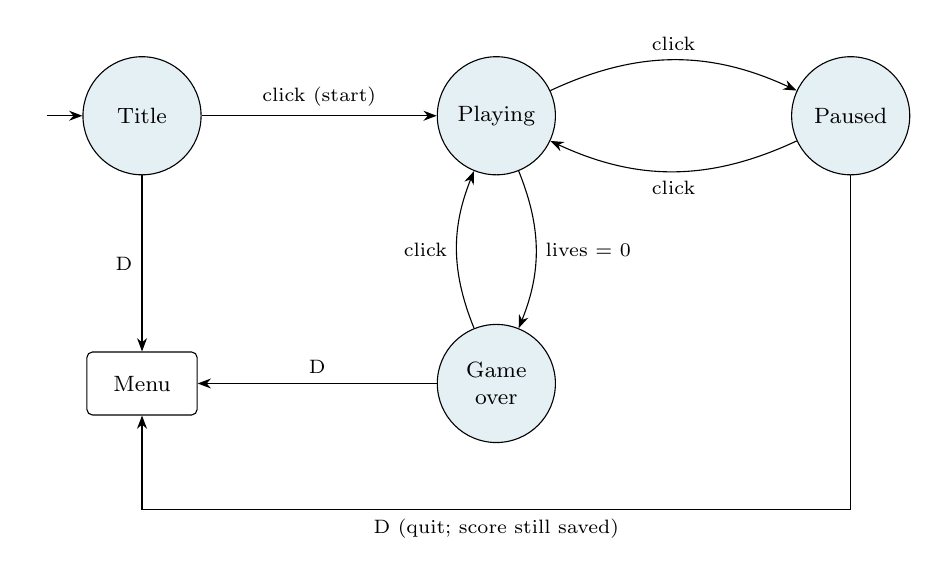
\begin{tikzpicture}[->, >=Stealth, auto]
  \node[state, initial, initial text=] (title) at (0,0) {Title};
  \node[state] (play)  at (4.5,0) {Playing};
  \node[state] (pause) at (9,0) {Paused};
  \node[state] (over)  at (4.5,-3.4) {Game\\over};
  \node[draw, rounded corners=2pt, font=\footnotesize, minimum width=14mm, minimum height=8mm] (menu) at (0,-3.4) {Menu};
  \path (title) edge node[above, font=\scriptsize]{click (start)} (play)
        (play)  edge[bend left=25] node[above, font=\scriptsize]{click} (pause)
        (pause) edge[bend left=25] node[below, font=\scriptsize]{click} (play)
        (play)  edge[bend left=22] node[right, font=\scriptsize]{lives = 0} (over)
        (over)  edge[bend left=22] node[left, font=\scriptsize]{click} (play)
        (title) edge node[left, font=\scriptsize]{D} (menu)
        (over)  edge node[above, font=\scriptsize]{D} (menu);
  \draw[->, >=Stealth] (pause.south) -- (9,-5.0) -- node[below, font=\scriptsize]{D (quit; score still saved)} (0,-5.0) -- (menu.south);
\end{tikzpicture}
\caption{Space Shooter state machine.}
\end{figure}

\paragraph{Physics.} With joystick input $u\in[-1,1]$, acceleration $a$, friction
coefficient $k$ and frame time $\Delta t$, each axis is updated as
\[
  v \leftarrow v + a\,u\,\Delta t,\qquad
  v \leftarrow v\,(1 - k\,\Delta t),\qquad
  |v| \le v_{\max},\qquad
  x \leftarrow x + v\,\Delta t.
\]
At full stick the speed would settle near $a/k = 550/2.5 = \unit{220}{px/s}$, so
the \unit{180}{px/s} limit is reached, which keeps the ship controllable.
$\Delta t$ is the measured time since the last frame (capped at 50\,ms), so
movement speed does not depend on frame rate.

\paragraph{Collisions.} Objects are treated as circles; two touch when
$d_x^2+d_y^2 < (r_1+r_2)^2$. Comparing squared distances avoids a square root.

\paragraph{Difficulty.} The asteroid spawn interval falls with score:
\[
  T_{\text{spawn}} = \max\big(300,\ 900 - 2\min(\text{score}, 300)\big)\ \text{ms}.
\]

\paragraph{Pause.} On resume, every stored timestamp (fire cooldowns, spawn
timers, shield end time, invulnerability, orb timer, banners) is shifted forward
by the pause length, so nothing expires or fires all at once.

\begin{longtable}{lr}
\caption{Space Shooter parameters.}\label{tab:shooterparams}\\
\toprule
\textbf{Parameter} & \textbf{Value} \\
\midrule\endfirsthead
\toprule
\textbf{Parameter} & \textbf{Value} \\
\midrule\endhead
Ship acceleration $a$ & 550\,px/s$^2$ \\
Friction $k$ & 2.5\,s$^{-1}$ \\
Maximum speed & 180\,px/s \\
Bullet speed & 300\,px/s \\
Fire cooldown per direction & 180\,ms ($\approx$5.6 shots/s) \\
Directions & A up, B right, D left \\
Asteroids (max on screen) & 10; radius 7--13\,px; speed 65--129\,px/s \\
Bullets (max) & 12 \\
Spawn interval & 900\,ms falling to 300\,ms \\
Points per asteroid & 10 \\
Lives & 3; 900\,ms invulnerability after a hit \\
Shield orb & every 5\,s; pickup radius 18\,px; up to 3 charges \\
Shield duration & 3\,s (button C) \\
Level banner & every 100 points \\
Particles & up to 64; life 0.35--0.7\,s \\
Starfield & 48 stars in 3 parallax layers (12, 30, 65\,px/s) \\
\bottomrule
\end{longtable}

\subsection{Snake}
\begin{figure}[H]
\centering
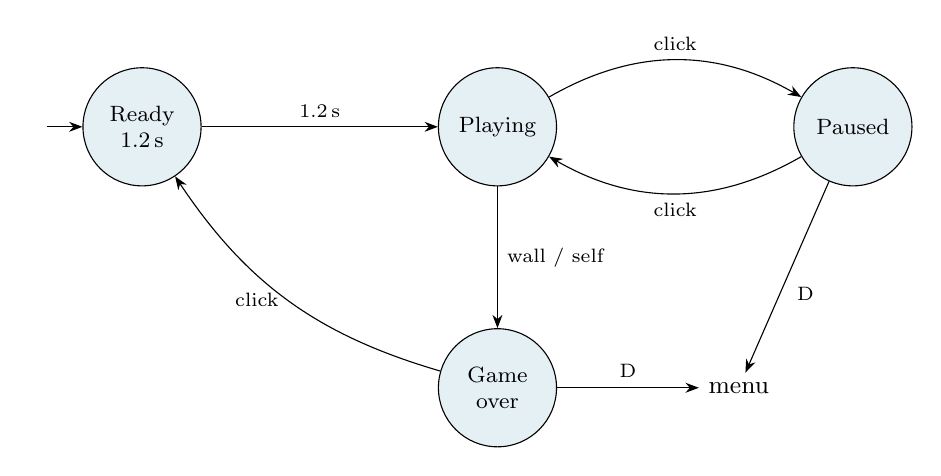
\begin{tikzpicture}[->, >=Stealth, node distance=30mm, auto]
  \node[state, initial, initial text=] (ready) {Ready\\1.2\,s};
  \node[state, right=of ready] (play) {Playing};
  \node[state, right=of play] (pause) {Paused};
  \node[state, below=18mm of play] (over) {Game\\over};
  \node[right=18mm of over, font=\small] (menu) {menu};
  \path (ready) edge node[font=\scriptsize]{1.2\,s} (play)
        (play) edge[bend left] node[font=\scriptsize]{click} (pause)
        (pause) edge[bend left] node[font=\scriptsize]{click} (play)
        (play) edge node[font=\scriptsize]{wall / self} (over)
        (over) edge[bend left=20] node[font=\scriptsize, left]{click} (ready)
        (over) edge node[font=\scriptsize]{D} (menu)
        (pause) edge node[font=\scriptsize]{D} (menu);
\end{tikzpicture}
\caption{Snake state machine.}
\end{figure}

\begin{table}[H]
\centering
\caption{Snake parameters.}
\begin{tabularx}{\linewidth}{lX}
\toprule
\textbf{Parameter} & \textbf{Value} \\
\midrule
Board & $32\times21$ cells of 10\,px (below a 30\,px HUD) \\
Move interval & 150\,ms, $-3$\,ms per apple, minimum 70\,ms \\
Points per apple & 10 \\
Maximum length & 672 cells \\
Turn rule & checked against the last \emph{executed} move, so two quick taps cannot reverse the snake into itself \\
\bottomrule
\end{tabularx}
\end{table}

\subsection{Display task (core 1)}
Core~1 has two states, \emph{Idle} (asleep in WFE) and \emph{Transferring}
(DMA running), switched by \texttt{transfer\_busy}.

% ==========================================================
\section{Measurements and Results}\label{sec:measure}
% ==========================================================

All numbers in this section were measured on the device, using the USB serial
log (one line per second) and the \texttt{benchmark\_test} program.

\subsection{CPU frequency}
See Table~\ref{tab:clocks}: 150\,MHz during operation, 48\,MHz in sleep.

\subsection{SPI speed}
See Table~\ref{tab:spi}: 75\,MHz operating clock (the RP2350 maximum), against an
80\,MHz request and a 62.5\,MHz panel rating; 63\,Mbit/s effective.

\subsection{Frame rate}\label{sec:fps}
\begin{table}[H]
\centering
\caption{Frame rate per screen and mode.}\label{tab:fps}
\begin{tabular}{lccc}
\toprule
\textbf{Screen} & \textbf{Single core} & \textbf{Dual core} & \textbf{Dual-core worst frame} \\
\midrule
Menu & 45 (predicted 44.4) & 51.4 & 19.5\,ms \\
Space Shooter (playing) & 47 & 51 & 19.5\,ms \\
Snake (playing) & 44 & 51 & 19.5\,ms \\
\bottomrule
\end{tabular}
\end{table}

\noindent Prediction: in single-core mode the frame time is render plus transfer,
so for the menu $1/(3.0+19.5)\,\text{ms} = 44.4$\,FPS. In dual-core mode it is
the larger of the two, $\max(3.0, 19.5) = 19.5$\,ms, giving 51.3\,FPS. The
measured 45\,FPS (single core) and 51.4\,FPS (dual core) match both predictions.
In both games the dual-core build also holds 51\,FPS, against 47 (Space Shooter)
and 44 (Snake) on one core. The dual-core gain, $51.4/45 = 1.14$ on the menu and
up to $51/44 = 1.16$ in Snake, is 9--16\,\% here
\emph{because drawing is so cheap}; the benefit grows with heavier scenes, until
drawing itself exceeds 19.5\,ms.

\subsection{CPU profile}\label{sec:profile}
\begin{table}[H]
\centering
\caption{Where the time goes per frame (dual core).}\label{tab:cpuprofile}
\begin{tabular}{lcccc}
\toprule
\textbf{Screen} & \textbf{Core 0 render} & \textbf{Core 0 wait} & \textbf{Core 0 load} & \textbf{Core 1 DMA} \\
\midrule
Menu & 3.0\,ms & 16.5\,ms & 15\,\% & 19.5\,ms \\
Space Shooter & 2.5\,ms & 17.0\,ms & 13\,\% & 19.5\,ms \\
Snake & 4.6\,ms & 14.8\,ms & 24\,\% & 19.5\,ms \\
\bottomrule
\end{tabular}
\end{table}

\noindent Core~0 load = render time / frame time. Snake costs the most to draw
(4.6\,ms) and Space Shooter the least (2.5\,ms), but even Snake leaves core~0
idle three quarters of the time. In every case the worst frame equals the
19.5\,ms transfer: drawing never makes a frame late. Core~1 spends almost the whole
frame supervising the DMA transfer; most of that time is a wait, not
computation.

\begin{table}[H]
\centering
\caption{Cost of individual operations (from \texttt{benchmark\_test}).}\label{tab:opcost}
\begin{tabular}{lc}
\toprule
\textbf{Operation} & \textbf{Time} \\
\midrule
\texttt{display\_clear} (full screen) & 1\,283\,\textmu s (16.7\,ns per pixel) \\
\texttt{fill\_rect} (full screen) & 1\,301\,\textmu s \\
\texttt{draw\_string} (19 characters) & 152\,\textmu s (8\,\textmu s per character) \\
\texttt{draw\_line} (full diagonal, 320 px) & 39.9\,\textmu s (125\,ns per pixel) \\
\texttt{fill\_circle} ($r=10$) & 19.1\,\textmu s \\
\texttt{fill\_triangle} (ship hull) & 26.9\,\textmu s \\
\texttt{gpio\_get} (incl.\ test loop) & 120.7\,ns \\
\texttt{joystick\_read\_x} & 3\,334\,ns \\
Full frame, clear + show (dual core) & 19\,461\,\textmu s (51.4\,FPS); DMA 19.5\,ms; core~0 wait 18.1\,ms \\
\bottomrule
\end{tabular}
\end{table}

\paragraph{Interpretation.} Clearing the framebuffer is the largest single
drawing cost (\unit{1.28}{ms}, about 2.5 cycles per pixel, roughly 43\,\% of the
menu's \unit{3.0}{ms} render time); writing two pixels per 32-bit store or
clearing with DMA could make it several times faster. Text is relatively
expensive because every lit glyph pixel is a separate clipped rectangle fill.
The \texttt{gpio\_get} figure includes the benchmark loop (a modulo and a
\texttt{volatile} write); the SIO pin read itself is one cycle (\unit{6.7}{ns}).
In the full-frame test core~0 works for $19.46 - 18.1 = \unit{1.36}{ms}$ (the
clear plus loop overhead) and waits for the rest: the frame time equals the DMA
time, confirming that the SPI link, not the CPU, limits the frame rate.

\paragraph{Interrupt load (estimate).} The two 1\,kHz interrupts each take a few
microseconds per call (entry and exit, a handful of pin reads or one PWM update),
about 2--4\,\textmu s per millisecond in total, i.e.\ under 0.5\,\% of core~0.

\subsection{Polling and update frequencies}
\begin{table}[H]
\centering
\caption{Polling frequencies.}\label{tab:polling}
\begin{tabularx}{\linewidth}{lrX}
\toprule
\textbf{Activity} & \textbf{Rate} & \textbf{Mechanism} \\
\midrule
Button sampling & 1\,kHz & Timer interrupt, core~0 \\
Sound engine update & 1\,kHz & Timer interrupt, core~0 \\
Button snapshot (\texttt{buttons\_poll}) & per frame, $\approx$51\,Hz & Main loop \\
Joystick ADC (X and Y) & per frame, $\approx$51\,Hz & Main loop \\
Idle check for auto-sleep & per frame on calm screens & Main loop \\
Wake check while asleep & 1\,kHz & Core~0 woken from WFI by the timer interrupt \\
FPS statistics / serial log & 1\,Hz & One-second window \\
Snake movement & 6.7--14.3\,Hz & 150\,ms falling to 70\,ms \\
Asteroid spawning & 1.1--3.3\,Hz & 900\,ms falling to 300\,ms \\
\bottomrule
\end{tabularx}
\end{table}

\subsection{Debounce and joystick timing}
Debounce: see Table~\ref{tab:inputtiming} (5\,ms, sampled at 1\,kHz). Joystick
reading: see Table~\ref{tab:adc}.

\subsection{Memory usage}
\begin{table}[H]
\centering
\caption{Memory usage (dual-core build).}\label{tab:mem}
\begin{tabular}{lrr}
\toprule
\textbf{Item} & \textbf{Bytes} & \textbf{Share} \\
\midrule
\multicolumn{3}{l}{\textit{Flash (4\,MB)}} \\
Firmware (code + constants) & 65\,196 (63.7\,KB) & 1.6\,\% \\
Saved scores sector & 4\,096 & 0.1\,\% \\
\midrule
\multicolumn{3}{l}{\textit{RAM (520\,KB)}} \\
Two framebuffers ($2\times153\,600$) & 307\,200 & 57.7\,\% \\
Space Shooter state, particles, stars, pop-ups & 3\,383 & 0.6\,\% \\
Snake body & 1\,344 & 0.3\,\% \\
Core~1 stack & 2\,048 & 0.4\,\% \\
USB stack, SDK and other & 3\,753 & 0.7\,\% \\
\textbf{Total static RAM} & \textbf{317\,728 (310.3\,KB)} & \textbf{59.7\,\%} \\
Free for heap (main SRAM) & $\approx$208\,600 (203.7\,KB) & 39.2\,\% \\
\bottomrule
\end{tabular}
\end{table}

\noindent The single-core build needs only one framebuffer and uses about
160\,KB of RAM. Dual-core rendering therefore costs 150\,KB of RAM in exchange
for overlapping drawing with transfer.

\subsection{Asset sizes}
Because sprites are procedural, the stored graphics and sounds are very small.
All of them are declared \texttt{const}, so they stay in flash and cost no RAM.

\begin{table}[H]
\centering
\caption{Asset sizes (from the firmware symbol table).}\label{tab:assets}
\begin{tabular}{lrl}
\toprule
\textbf{Asset} & \textbf{Bytes} & \textbf{Content} \\
\midrule
5$\times$7 font & 195 & 39 glyphs $\times$ 5 columns \\
Heart icon & 6 & 7$\times$6 bitmap \\
Sound-effect segments & 120 & 15 segments $\times$ 8\,B \\
Sound-effect descriptors & 80 & 10 effects $\times$ 8\,B \\
Menu game table & 32 & 2 games $\times$ 16\,B \\
Button pin table & 20 & 5 pins \\
\textbf{Total stored assets} & \textbf{453} & \\
\midrule
Ship, asteroids, orb, snake, icons & 0 & drawn procedurally in code \\
Note frequencies (\file{notes.h}) & 0 & compile-time constants \\
\bottomrule
\end{tabular}
\end{table}

% ==========================================================
\section{Testing and Validation}
% ==========================================================
\begin{itemize}
  \item \textbf{Hardware tests}: each part has a stand-alone program.
        \texttt{display\_test} (border, colour bars, moving square, FPS),
        \texttt{buttons\_test} (state plus a press counter that must rise by
        exactly 1 per press, demonstrating the debounce), \texttt{joystick\_test}
        (raw and normalised values, for calibration), \texttt{sound\_test}
        (scale and sweep), and \texttt{benchmark\_test} (all timing figures).
  \item \textbf{Flash save logic}: tested on a PC against a simulated flash chip
        (Section~\ref{sec:save}).
  \item \textbf{Rendering}: early UI frames were rendered on a PC with stubbed
        hardware and inspected as images.
  \item \textbf{Code quality}: every source file compiles with
        \texttt{-Wall -Wextra -Wshadow} with zero warnings.
  \item \textbf{On device}: FPS and timing logged over USB; sleep/wake, pause and
        score persistence across power cycles checked by hand.
\end{itemize}

% ==========================================================
\section{Limitations and Future Work}
% ==========================================================
\begin{itemize}
  \item \textbf{Not implemented}: enclosure, multi-console play.
        Multi-console play could use a UART link between two handhelds (three
        wires: TX, RX, ground) exchanging game state each frame.
  \item \textbf{SPI bandwidth limits FPS} to about 51. Options: redraw only the
        parts of the screen that changed (dirty rectangles), 16-bit DMA transfers,
        or the RP2350's programmable I/O (PIO) to drive the panel.
  \item \textbf{Backlight always on}: wiring BL to a GPIO would allow switching it
        off in sleep and PWM brightness control.
  \item \textbf{Sound}: one voice only (no chords) and a square-wave timbre; a
        low-pass filter or a PWM-based DAC would soften the tone and allow
        software volume control.
  \item \textbf{Joystick}: the dead zone causes a small jump in output at its
        edge; rescaling and auto-calibrating the centre at boot would smooth
        control.
\end{itemize}

% ==========================================================
\section{Conclusion}
% ==========================================================
The project delivers a working Pico~2 handheld with a menu and two complete
games. It meets the core software requirements with framebuffer rendering,
measured FPS, persistent scores, debounced input and dual-core operation, and
adds DMA transfers, non-blocking sound, physics, pause and sleep. The main
performance result is that the dual-core pipeline lets the display run at the
maximum rate the SPI link allows, about 51\,FPS, while core~0 stays about 85\,\%
idle. The main remaining work is physical: the enclosure.

% ==========================================================
\appendix
\section{Building and Flashing}
\begin{lstlisting}[language=bash]
cmake -S . -B build                    # board: pico2 (RP2350)
cmake --build build --target handheld  # firmware -> build/handheld.uf2

# single-core comparison build
cmake -S . -B build -DHANDHELD_DUAL_CORE=OFF

# flash with picotool, or hold BOOTSEL and copy the .uf2 to the RP2350 drive
picotool load -f build/handheld.uf2 && picotool reboot
\end{lstlisting}

\section{Controls}
\begin{center}\small
\begin{tabularx}{\linewidth}{lXXX}
\toprule
\textbf{Input} & \textbf{Menu} & \textbf{Space Shooter} & \textbf{Snake} \\
\midrule
Joystick & Choose game & Move ship & Steer \\
A & Hold 3\,s: reset scores & Fire up & Up \\
B & Next game & Fire right & Right \\
C & FPS overlay & Shield & Down \\
D & Previous game & Fire left; menu on title/pause/game over & Left; menu on pause/game over \\
Click & Tap: play; hold 2\,s: sleep & Start; pause/resume & Pause/resume; play again \\
\bottomrule
\end{tabularx}
\end{center}

\section{Glossary}
\begin{longtable}{lp{11.5cm}}
\toprule
\textbf{Term} & \textbf{Meaning} \\
\midrule\endhead
ADC & Analog-to-digital converter: turns a voltage into a number \\
CRC32 & 32-bit cyclic redundancy check: a checksum that detects corrupted data \\
DMA & Direct memory access: hardware that copies data without the CPU \\
DMB & Data memory barrier: an instruction that orders memory accesses \\
DREQ & Data request: a peripheral's signal telling the DMA it is ready for more data \\
FPS & Frames per second \\
FPU & Floating-point unit \\
GRAM & Graphics RAM inside the display controller \\
ISR & Interrupt service routine: code run when an interrupt fires \\
LFSR & Linear-feedback shift register: a fast pseudo-random number generator \\
Mux & Multiplexer: a switch that selects one of several inputs \\
PLL & Phase-locked loop: multiplies a reference clock to a higher frequency \\
PWM & Pulse-width modulation: a square wave with adjustable frequency and duty cycle \\
RGB565 & 16-bit colour: 5 bits red, 6 green, 5 blue \\
SEV / WFE & Send event / wait for event: inter-core signalling instructions \\
SIO & Single-cycle I/O: per-core block for fast GPIO and inter-core signals \\
SPI & Serial Peripheral Interface: a clocked serial bus \\
WFI & Wait for interrupt: halts the core until an interrupt arrives \\
XIP & Execute-in-place: running code directly from flash \\
\bottomrule
\end{longtable}



\end{document}
